\documentclass[letterpaper]{article}

\usepackage{graphicx}
\usepackage[letterpaper, left=30mm, right=30mm, top=30mm, bottom=30mm]{geometry}

\begin{document}

\begin{flushright}
	
\includegraphics[width=5cm, height=4cm]{Imagenes/logoMATCOM.png}\\
	{\scriptsize \textbf{Facultad de Matemática y Computación}}
\end{flushright}

\

\

\begin{center}
	\textbf{{\Huge PROYECTO DE }}
	
	\

	\textbf{{\Huge PROGRAMACIÓN II}}
	\

	\

	\

	\

	\

	\

	\

	\

	\

	\textbf{{\Huge H U L K}}

	\
	
	\textbf{{\LARGE Havana University Language for Kompilers}}
\end{center}

\begin{figure}[b]
	\begin{flushleft}
		{\huge \textbf{Estudiante:} \textit{Claudia Hernández Pérez}}

		\
	
		{\LARGE \textbf{Grupo:} \textit{C-113}}
	\end{flushleft}
\end{figure}

\newpage
{\small
HULK es un lenguaje de programación imperativo, funcional, estática y fuertemente tipado. Casi todas las instrucciones en HULK son expresiones. 
En particular, el subconjunto de HULK que usted implementar se compone solamente de expresiones que pueden escribirse en una línea. \\

\textbf{{\large $\circ $  Tipos Básicos}}\\

El lenguaje HULK contiene tres tipos básicos: 'string', 'boolean' y 'number'.

\begin{center}
	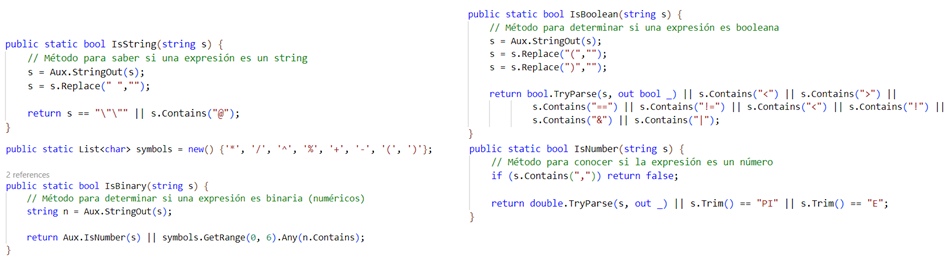
\includegraphics[width=13cm, height=4.25cm]{Imagenes/Types.png}\\
	{\scriptsize \textbf{Fig 1.1 Identificación de tipos básicos del lenguaje}}
\end{center}

La jerarquía de símbolos es: \\
• Símbolos de tipo 'number' : $\wedge$'; '*', '/' y '\%'; '+' y '-' \\
• Símbolos de tipo 'boolean':  '!'; '$>$', '$<$', '$>=$' y '$<=$'; '==' y '!='; '\&' y '$|$' \\
• Símbolos de tipo 'string' : '@' \\

De forma recursiva se procede en sentido contrario a la jerarquía, de forma que se va descomponiendo la expresión desde la operación más interna a la más externa.
La expresión se va evualuando en dos miembros, excepto el '!' que solo admite miembro derecho, haciéndola tan pequeña hasta que se llegue a la operación que según la 
jerarquía deba ejecutarse primero.

\begin{center}
\end{center}


\textbf{{\large $\circ $ Funciones}}\\

Una función en el HULK solo es posible definirla con la palabra 'function' al inicio de la expresión. El cuerpo de una función admite cualquier expresión válida en 
el lenguaje. Debe respetarse la sintaxis:
\begin{center}
	function nombre(variables) $=>$ cuerpo;
\end{center}

Además de las funciones que el usuario desee crear, el lenguaje cuenta con una gama de funciones predefinidas: \\
• cos(x) $=>$ calcula el coseno de 'x' \\
• sin(x) $=>$ calcula el seno de 'x' \\
• tg(x) $=>$ calcula la tangente de 'x' \\
• sqrt(x) $=>$ calcula la raíz cuadrada de 'x' \\
• log(x, y) $=>$ calcula el logaritmo de 'y' en base de 'x', si no se da el argumento 'y' entonces se calcula el logaritmo natural de 'x'  \\
• exp(x) $=>$ calcula $e ^ x$ \\
• rand(x) $=>$ devuelve un número random entre 0 y 1 \\


\textbf{{\large $\circ $ Variables}}\\

También es posible declarar variables con la instrucción 'let-in', donde se pueden declarar más de una, en ese caso separadas por ','. La forma más
simple de esta instrucción es: 

\begin{center}
	let variable = value in cuerpo;
\end{center}

Así como es posible declarar más de una variable, se pueden declarar más de un 'let-in' de la forma:

\begin{center}
	let variable1 = value in (let variable2 = value in cuerpo);
\end{center}

En este último es posible que en el cuerpo intervengan ambas variables o incluso la segunda dependa de la primera.
Un dato a destacar es que las variables que se definan bajo esta instrucción dejarán de existir cuando se devuelva 
el valor de su evaluación y, al igual que en las funciones, es posible declarar en el 'cuerpo' cualquier expresión
válida en el lenguaje. \\

\textbf{{\large $\circ $ Condicionales}} \\

Las condiciones en el lenguaje son bajo la instrucción 'if-else', que consta de tres partes: la condición, el cuerpo 
de evaluar true y el cuerpo de evaluar false, de la forma:

\begin{center}
	if (condición) cuerpo true else cuerpo false;
\end{center}

Como en el 'let-in', en las condiciones se pueden identar unas dentro de otras. \\

\textbf{{\large $\circ $ Recursión}} \\

Dado que en el lenguaje es posible definir funciones y condiciones, soporta también la definición de funciones recursivas.
La sintaxis básica de estas puede parecerse a:

\begin{center}
	function nombre(variables) => if (condición de stop) retorno else llamado recursivo;
\end{center}

En la recursión se manejarán problemas de 'Stack Overflow' en la ejecución si no se declara condición de parada correcta
o si se desborda. \\

\textbf{{\large $\circ $ Errores}}\\

En el proyecto se destinó una clase exclusivamente para revisar todos los posibles errores de las expresiones en en lenguaje.
Desde errores más básicos como la falta de un miembro en una expresión básica o que el valor dado no corresponda con el tipo
que se espera para realizar la operación. De las instrucciones se verifica que hayan sido definidas todas sus partes correctamente. 
Hasta elementos que no son reconocidos por ninguno de los tipos definidos que son clasificados como expresiones inválidas.

Hay 4 tipos de errores: \\
• Léxico : Verifica que ciertos elementos cumplan con las reglas de escritura reglamentadas. \\
• Sintáctico : Verifica expresiones mal formadas como paréntesis no balanceados o expresiones incompletas. \\
• Semántico : Verifica el uso incorrecto de los tipos y argumentos. \\
• Ejecución : Solamente está definido el 'Stack Overflow' por funciones recursivas. \\

En caso de haber sido detectado un error se imprime en pantalla y se detiene la evaluación, para el control de que solamente
se imprima uno se verifica una variable booleana estática que solo es true si ya fue identificado un error. \\

\textbf{{\large $\circ $ Algunos detalles de implementación}}\\

• Cada expresión tiene carácter obligatorio terminar en ';'.

\

• En los strings serán reconocidos los códigos con un backslash delante: 'n', 'r', 't', 'a', 'f', 'b', 'v'.

\

• En el caso de las condicionales, cuando están identadas el lenguaje reconoce tanto 'else if' como 'elif'.

\

• En las funciones predefinidas se verifica que cumpla con reglas como el 'log' y la raíz cuadrada. 

\

• Para la recursividad fue creada una caché para guardar los valores ya calculados.

\

• El 'Stack Overflow' es dado cuando las llamadas a la función alcanzan las 250. 
}

\end{document}